\documentclass{article}
\usepackage[utf8]{inputenc}
\usepackage[greek,english]{babel}
\usepackage{alphabeta}
\usepackage{fancyhdr}
\usepackage{listings}
\usepackage{mathtools}
\usepackage{xcolor}
\usepackage{biblatex}
\usepackage[left=2cm,right=2cm]{geometry}

\lstset {
        basicstyle=\ttfamily,
        columns=fullflexible,
        breaklines=true,
        keepspaces=true
}

\title{Σχεδίαση Ψηφιακών Συστημάτων - Εργασία Θεωρίας (Μέρος 4)}
\author{Χρήστος Μαργιώλης}
\date{Ιούλιος 2020}

\begin{document}

\begin{titlepage}
        \maketitle
\end{titlepage}

\renewcommand{\contentsname}{Περιεχόμενα}
\tableofcontents

\section{Κώδικας και τεκμηρίωση}

\subsection{\lstinline{ctrl.vhd}}

Το παρακάτω κύκλωμα υλοποιεί την μονάδα ελέγχου ενός επεξεργαστή. Η υλοποίηση
έγινε με βάση τον πίνακα από τις διαφάνειες του μαθήματος. Στο τέλος προτίμησα
την δομή \lstinline{with-select} για πιο ευανάγνωστο κώδικα. \\

\lstinputlisting[language=VHDL]{../ctrl.vhd}
\pagebreak

\subsection{\lstinline{ctrl_tb.vhd}}

Testbench για την μονάδα ελέγχου. \\

\lstinputlisting[language=VHDL]{../ctrl_tb.vhd}
\pagebreak

\subsection{\lstinline{sign_ext.vhd}}

Το παρακάτω κύκλωμα υλοποιεί την μονάδα επέκτασης προσήμου. Στην αρχιτεκτονική
της, ορίζουμε την έξοδο σε (\lstinline{XXXX} συμβολίζει την είσοδο instruction):
\begin{itemize}
	\item \lstinline{0x0000XXXX} όταν το MSB του instruction ειναι 0.
	\item \lstinline{0xffffXXXX} όταν το MSB είναι 1. \\
\end{itemize}

\lstinputlisting[language=VHDL]{../sign_ext.vhd}
\pagebreak

\subsection{\lstinline{sign_ext_tb.vhd}}

Testbench για την μονάδα επέκτασης προσήμου. \\

\lstinputlisting[language=VHDL]{../sign_ext_tb.vhd}
\pagebreak

\subsection{\lstinline{shl2.vhd}}

Το παρακάτω κύκλωμα υλοποιεί μία μονάδα αριστερής ολίσθησης κατά 2 bit. Η
αρχιτεκτονική της είναι πολύ απλή: παίρνουμε τα 30 τελευταία bit της εισόδου
και τους «κολλάμε» (concatenate) 2 μηδενικά bit στο τέλος. \\

\lstinputlisting[language=VHDL]{../shl2.vhd}
\pagebreak

\subsection{\lstinline{shl2_tb.vhd}}

Testbench για την μονάδα αριστερής ολίσθησης κατά 2 bit. \\

\lstinputlisting[language=VHDL]{../shl2_tb.vhd}
\pagebreak

\section{Εκτέλεση}

\subsection{\lstinline{ctrl_tb}}
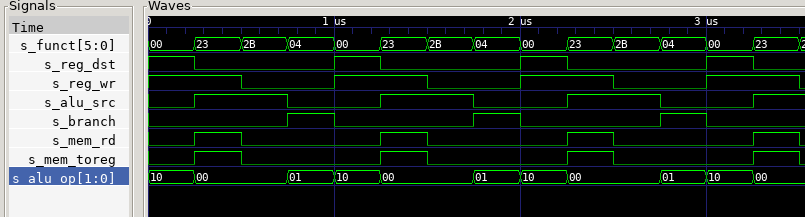
\includegraphics[width=\textwidth]{res/ctrl.png}

\subsection{\lstinline{sign_ext_tb}}
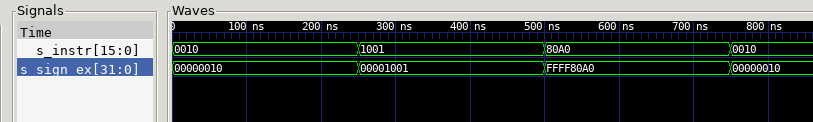
\includegraphics[width=\textwidth]{res/sign_ext.png}

\subsection{\lstinline{shl2_tb}}
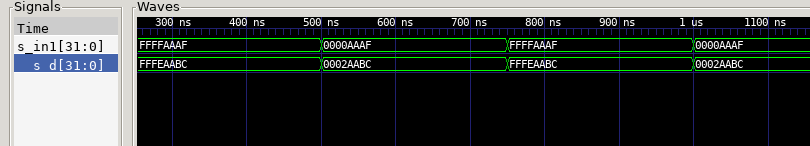
\includegraphics[width=\textwidth]{res/shl2.png}

\end{document}
